\documentclass[tikz,border=8pt]{standalone}
\usepackage[T1]{fontenc}
\usepackage{tikz}
\usetikzlibrary{arrows.meta,positioning,calc,decorations.pathreplacing}

\begin{document}
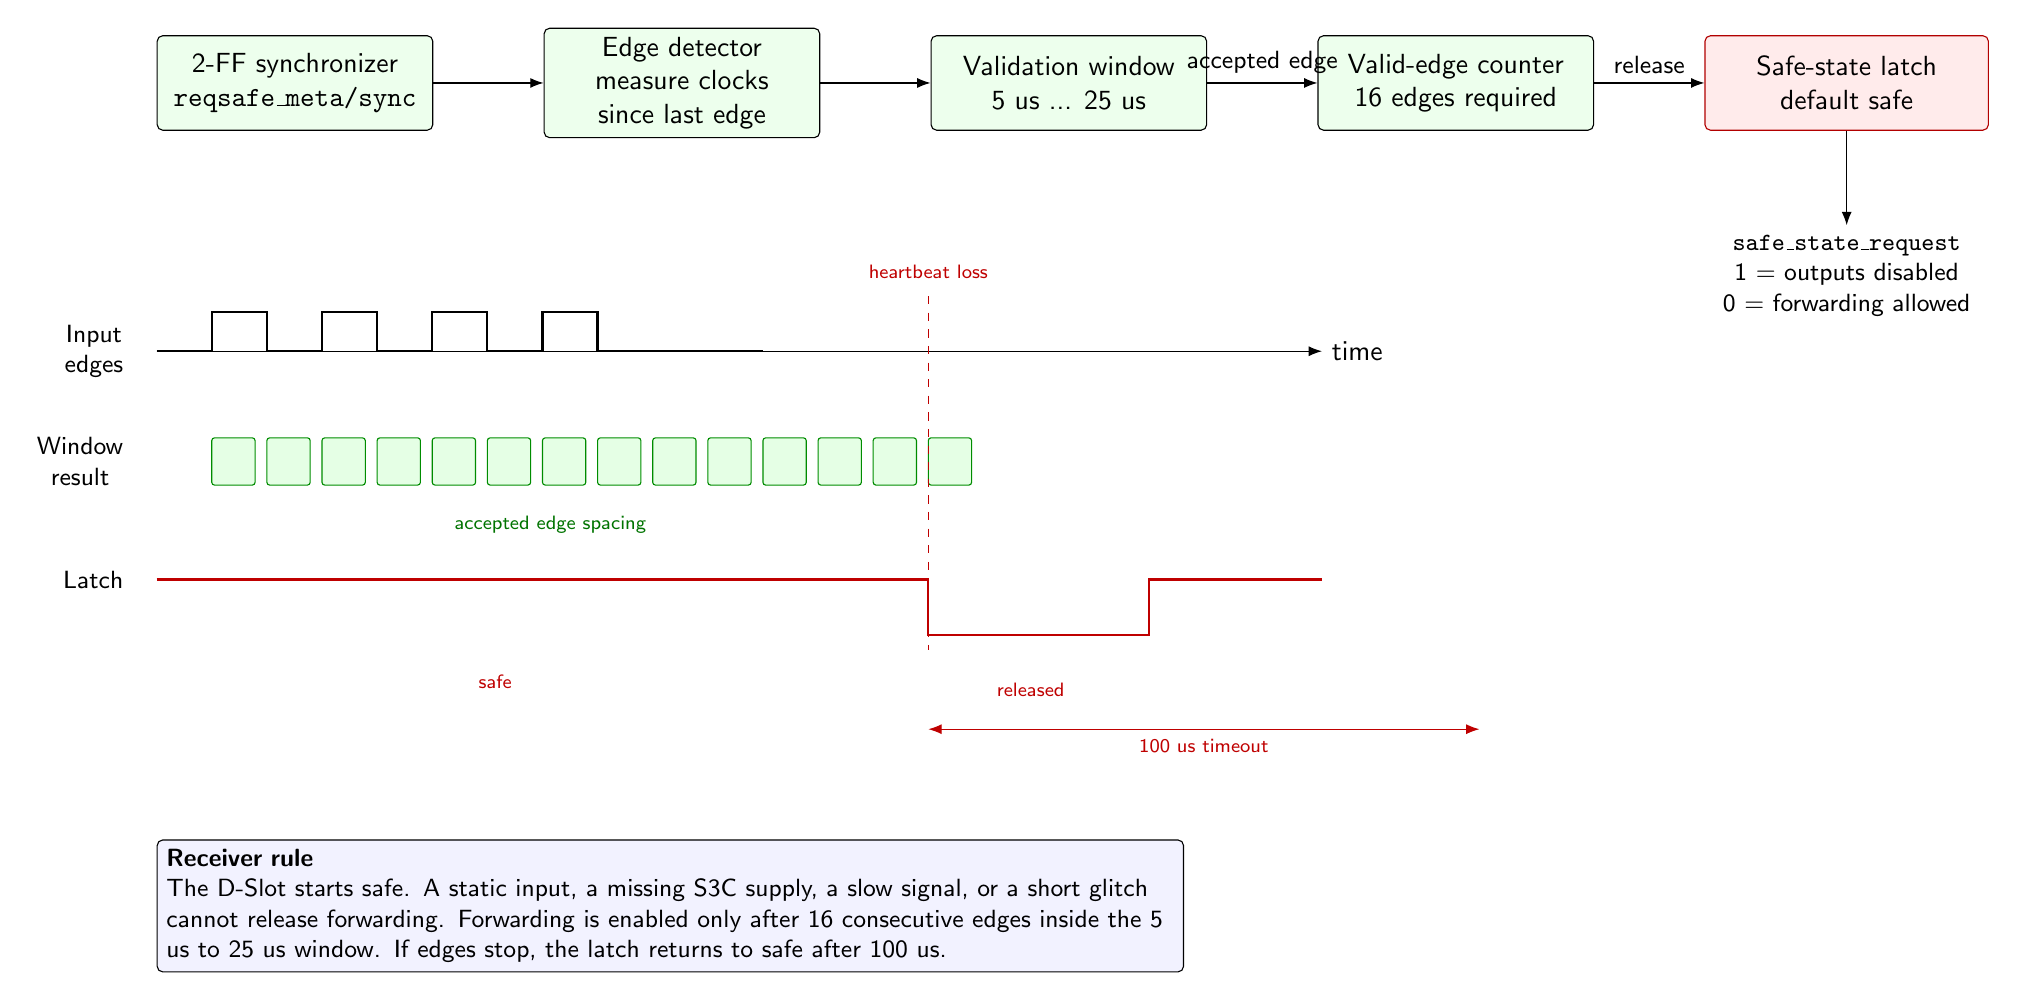
\begin{tikzpicture}[
  font=\sffamily,
  >=Latex,
  block/.style={draw, rounded corners=2pt, align=center, minimum height=12mm, minimum width=35mm, fill=green!7},
  latch/.style={draw=red!70!black, fill=red!8, rounded corners=2pt, align=center, minimum height=12mm, minimum width=36mm},
  note/.style={align=center, font=\sffamily\small},
  tinytext/.style={align=center, font=\sffamily\scriptsize},
  good/.style={draw=green!55!black, fill=green!10, rounded corners=1pt},
  bad/.style={draw=red!70!black, fill=red!9, rounded corners=1pt},
  sig/.style={thick}
]

\node[block] (sync) {2-FF synchronizer\\\texttt{reqsafe\_meta/sync}};
\node[block, right=14mm of sync] (edge) {Edge detector\\measure clocks\\since last edge};
\node[block, right=14mm of edge] (window) {Validation window\\5 us ... 25 us};
\node[block, right=14mm of window] (counter) {Valid-edge counter\\16 edges required};
\node[latch, right=14mm of counter] (latch) {Safe-state latch\\default safe};

\draw[->] (sync) -- (edge);
\draw[->] (edge) -- (window);
\draw[->] (window) -- node[above,note] {accepted edge} (counter);
\draw[->] (counter) -- node[above,note] {release} (latch);

\node[note, below=12mm of latch] (out) {\texttt{safe\_state\_request}\\1 = outputs disabled\\0 = forwarding allowed};
\draw[->] (latch) -- (out);

\coordinate (t0) at ($(sync.south west)+(0,-28mm)$);
\draw[->] (t0) -- ++(148mm,0) node[right] {time};
\node[note, anchor=east] at ($(t0)+(-3mm,0mm)$) {Input\\edges};
\node[note, anchor=east] at ($(t0)+(-3mm,-14mm)$) {Window\\result};
\node[note, anchor=east] at ($(t0)+(-3mm,-29mm)$) {Latch};

\draw[sig] ($(t0)+(0,0)$)
  -- ++(7mm,0) -- ++(0,5mm) -- ++(7mm,0) -- ++(0,-5mm)
  -- ++(7mm,0) -- ++(0,5mm) -- ++(7mm,0) -- ++(0,-5mm)
  -- ++(7mm,0) -- ++(0,5mm) -- ++(7mm,0) -- ++(0,-5mm)
  -- ++(7mm,0) -- ++(0,5mm) -- ++(7mm,0) -- ++(0,-5mm)
  -- ++(21mm,0);

\foreach \x in {7,14,21,28,35,42,49,56,63,70,77,84,91,98} {
  \draw[good] ($(t0)+(\x mm,-17mm)$) rectangle ++(5.5mm,6mm);
}
\node[tinytext, green!45!black] at ($(t0)+(50mm,-22mm)$) {accepted edge spacing};

\draw[sig, red!75!black] ($(t0)+(0,-29mm)$) -- ++(98mm,0)
  -- ++(0,-7mm) -- ++(28mm,0)
  -- ++(0,7mm) -- ++(22mm,0);
\node[tinytext, red!75!black] at ($(t0)+(43mm,-42mm)$) {safe};
\node[tinytext, red!75!black] at ($(t0)+(111mm,-43mm)$) {released};

\draw[dashed, red!75!black] ($(t0)+(98mm,7mm)$) -- ($(t0)+(98mm,-38mm)$);
\node[tinytext, red!75!black, anchor=south] at ($(t0)+(98mm,8mm)$) {heartbeat loss};
\draw[<->, red!75!black] ($(t0)+(98mm,-48mm)$) -- node[below,tinytext] {100 us timeout} ($(t0)+(168mm,-48mm)$);

\node[draw, rounded corners=2pt, fill=blue!5, align=left, font=\sffamily\small, anchor=north west, text width=128mm]
  at ($(t0)+(0mm,-62mm)$) {
  \textbf{Receiver rule}\\
  The D-Slot starts safe. A static input, a missing S3C supply, a slow signal, or a short glitch
  cannot release forwarding. Forwarding is enabled only after 16 consecutive edges inside the
  5 us to 25 us window. If edges stop, the latch returns to safe after 100 us.
  };

\end{tikzpicture}
\end{document}
